% CVPR 2023 Paper Template
% based on the CVPR template provided by Ming-Ming Cheng (https://github.com/MCG-NKU/CVPR_Template)
% modified and extended by Stefan Roth (stefan.roth@NOSPAMtu-darmstadt.de)

\documentclass[10pt,twocolumn,letterpaper]{article}

%%%%%%%%% PAPER TYPE  - PLEASE UPDATE FOR FINAL VERSION
\usepackage[review]{cvpr}      % To produce the REVIEW version
%\usepackage{cvpr}              % To produce the CAMERA-READY version
%\usepackage[pagenumbers]{cvpr} % To force page numbers, e.g. for an arXiv version

% Include other packages here, before hyperref.
\usepackage{graphicx}
\usepackage{amsmath}
\usepackage{amssymb}
\usepackage{booktabs}


% It is strongly recommended to use hyperref, especially for the review version.
% hyperref with option pagebackref eases the reviewers' job.
% Please disable hyperref *only* if you encounter grave issues, e.g. with the
% file validation for the camera-ready version.
%
% If you comment hyperref and then uncomment it, you should delete
% ReviewTempalte.aux before re-running LaTeX.
% (Or just hit 'q' on the first LaTeX run, let it finish, and you
%  should be clear).
\usepackage[pagebackref,breaklinks,colorlinks]{hyperref}


% Support for easy cross-referencing
\usepackage[capitalize]{cleveref}
\crefname{section}{Sec.}{Secs.}
\Crefname{section}{Section}{Sections}
\Crefname{table}{Table}{Tables}
\crefname{table}{Tab.}{Tabs.}


%%%%%%%%% PAPER ID  - PLEASE UPDATE
\def\cvprPaperID{*****} % *** Enter the CVPR Paper ID here
\def\confName{CVPR}
\def\confYear{2023}


\begin{document}

%%%%%%%%% TITLE - PLEASE UPDATE
\title{\LaTeX\ Author Guidelines for \confName~Proceedings}


\author{Daheng Yin, Mengyang Liu, Baijun Chen, Fang Dong\\
School of Computer Science and Engineering, Southeast University, Nanjing, China\\
{\tt\small \{yindaheng98, myliu, bjchen, fdong\}@seu.edu.cn}
}
\maketitle

%%%%%%%%% ABSTRACT
\begin{abstract}
   The ABSTRACT 
\end{abstract}

%%%%%%%%% BODY TEXT
\section{Introduction}
\label{sec:intro}

Introduction of efficient super resolution.

Designing an efficient model is non-trivial and always tedious. On one hand, lots of existing work look for insights for reducing FLOPs on operations but which always ignoring realistic execution on chip. On the other hand, the macro architecture design of model is also important such as using multiple connection, multiple resolution and local sharing. The space to designing a SOTA model is too large and it's always fatigued to update model with complex design over and over.

In this paper, we proposed a model-scaling based method to generate a more efficient model structure by an automatic procedure: first expanding and then shrinking.\ref{fig:overview}

Introduction of evaluation results.

The main contributions of this work are as follows:

\begin{itemize}
    \item Discussing on how to design an efficient model in an automatic way.
    \item Proposing \"Expand Big, Then Shrink\" method to automatic adapting an old SOTA model to a new bigger dataset which is an efficient way to design new model.
    \item Evaluating our method on main stream datasets and compared our results with other peers in NTIRE-ESRX4 challenge.
\end{itemize}

\begin{figure}[t]
  \centering
  % \fbox{\rule{0pt}{2in} \rule{0.9\linewidth}{0pt}}
   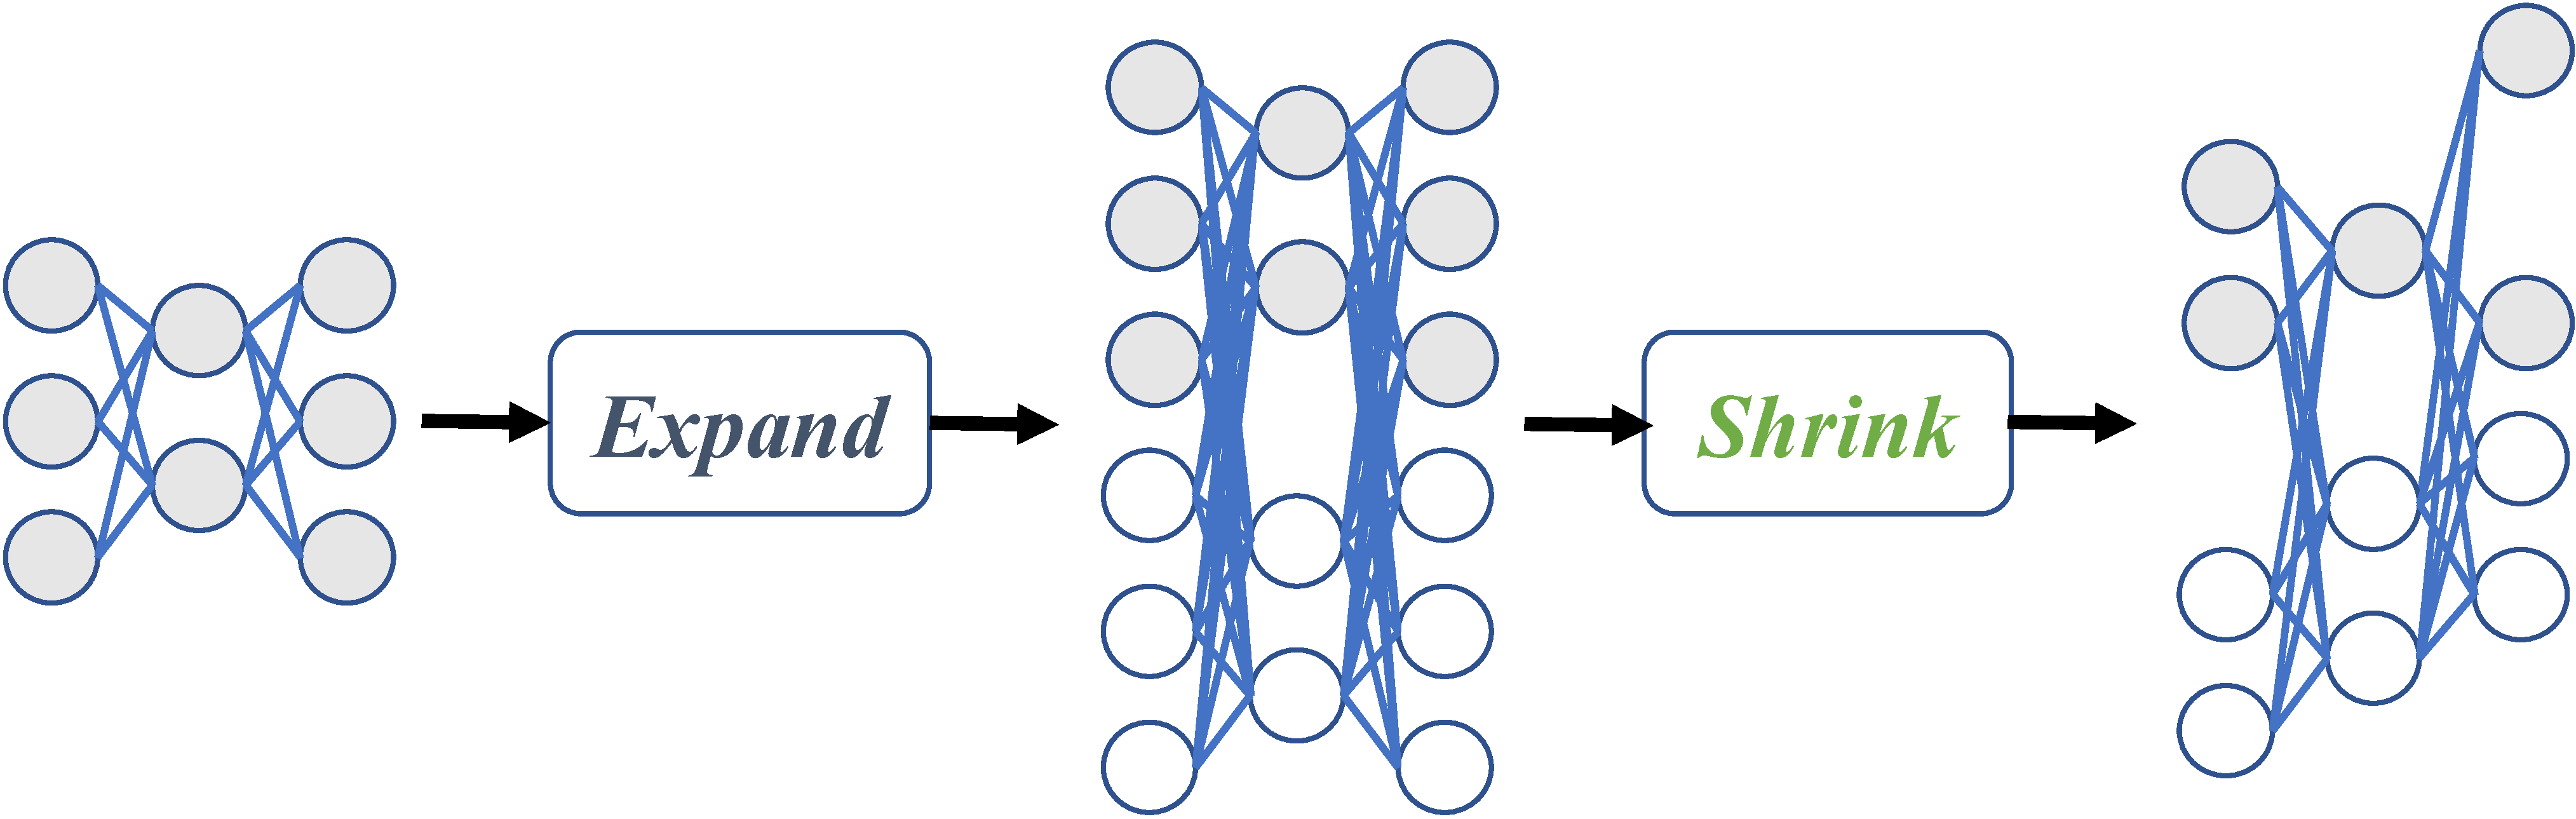
\includegraphics[width=0.8\linewidth]{../expandandshrink.pdf}

   \caption{Designing and training a SOTA model is a non-trivial work. Our work shows that expanding an existing model and then shrink it by pruning and finetuning is an efficient way to improve the performance of model.}
   \label{fig:overview}
\end{figure}



%------------------------------------------------------------------------
\section{Related Work}
\label{sec:related}

Related work.


%------------------------------------------------------------------------
\section{Method}
\label{sec:method}

\begin{figure*}
    \centering
    \begin{subfigure}[b]{0.49\linewidth}
		\centering
        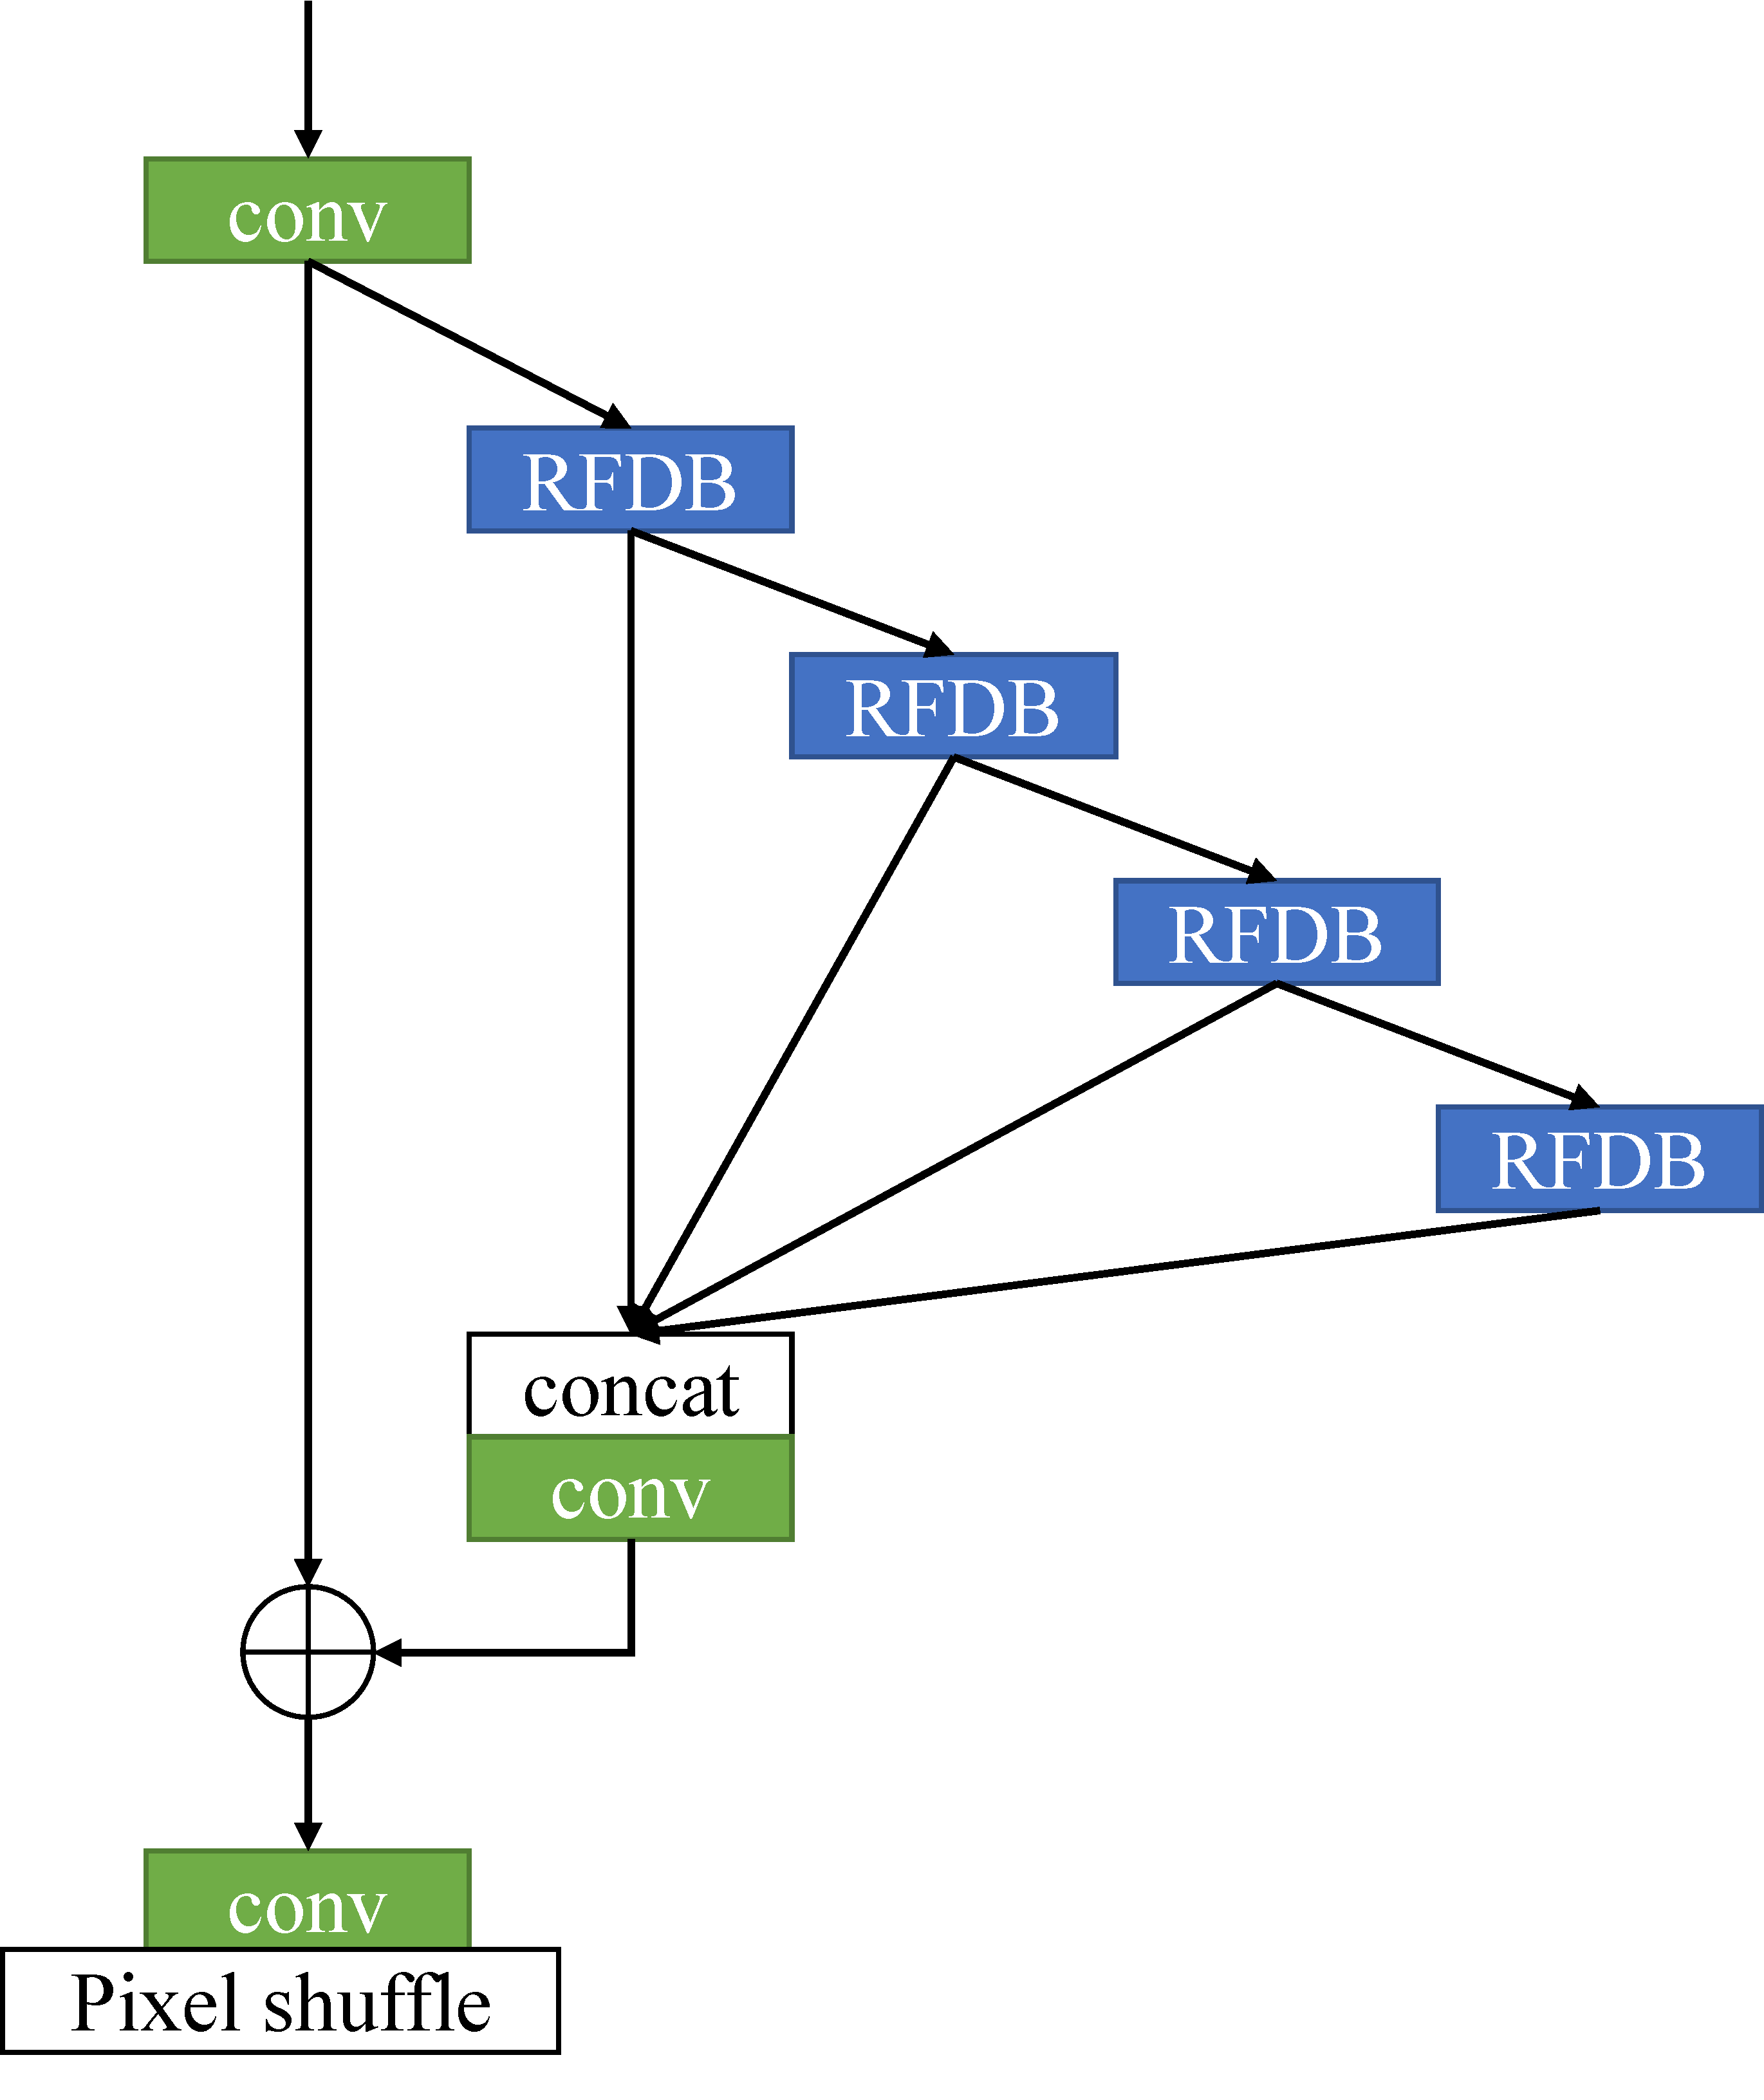
\includegraphics[width=\textwidth]{../RFDN.pdf}
        \caption{RFDN}
        \label{fig:RFDN}
    \end{subfigure}
    \begin{subfigure}[b]{0.49\linewidth}
		\centering
        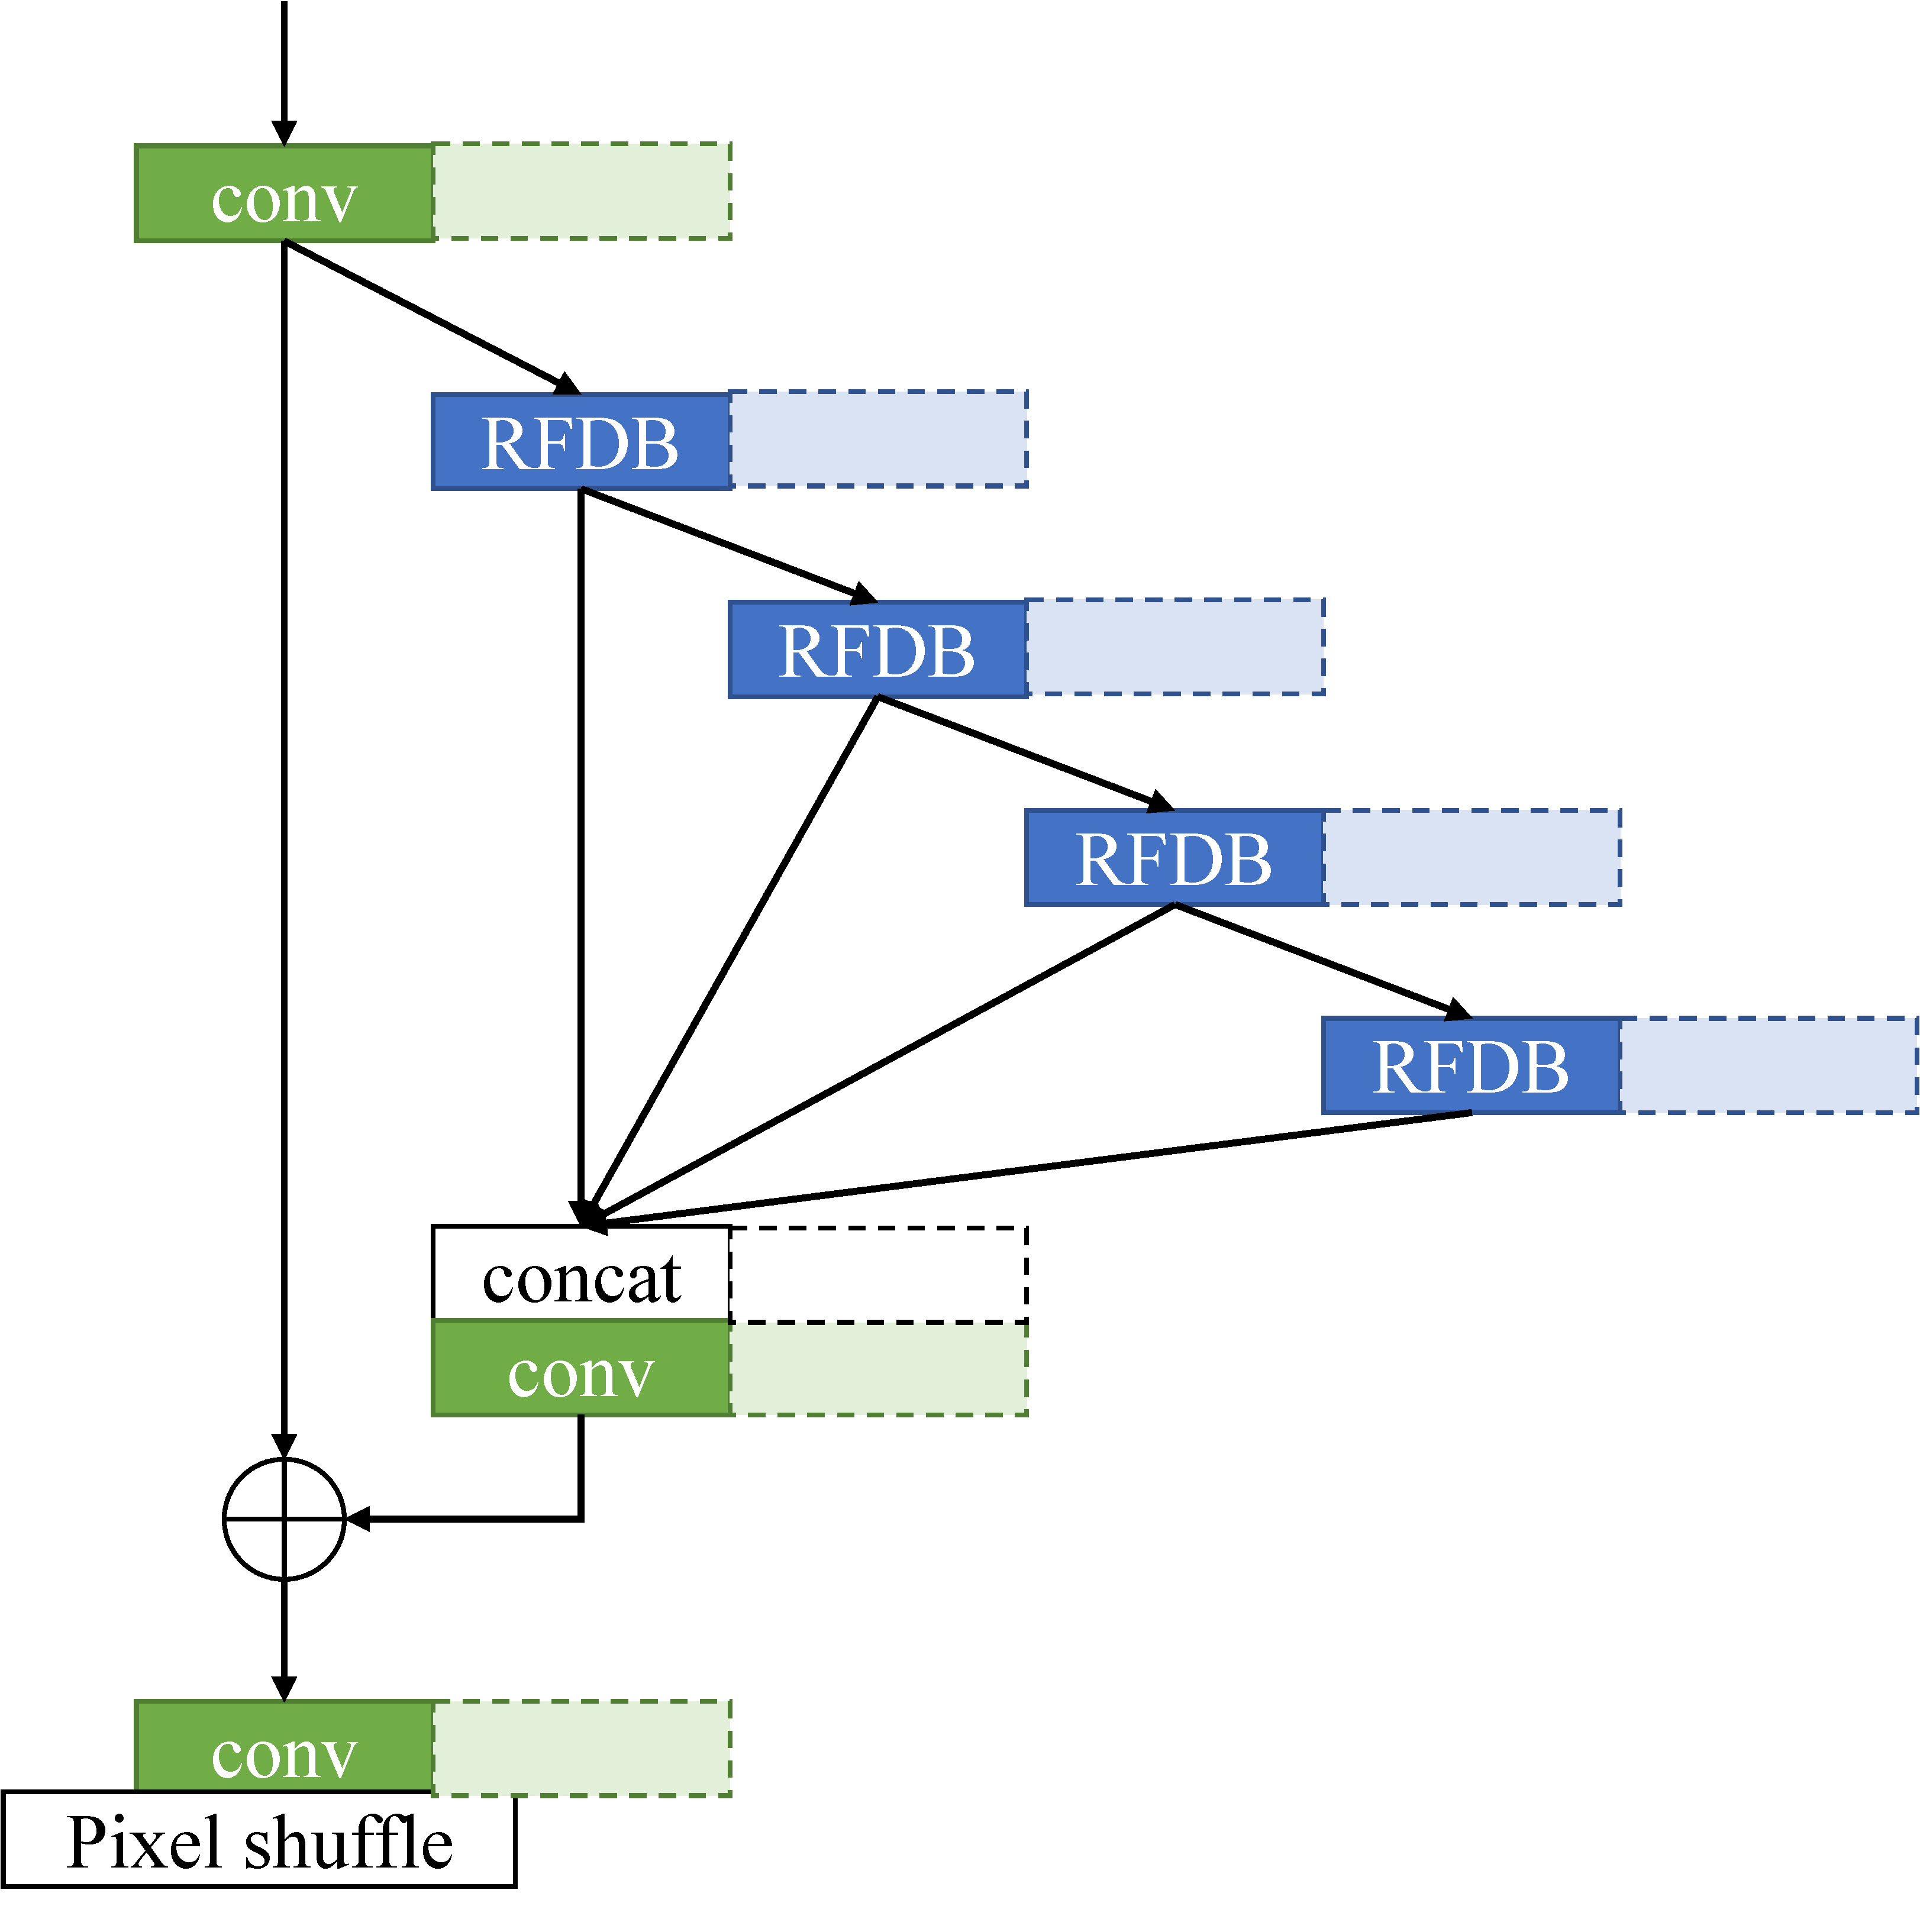
\includegraphics[width=\textwidth]{../expand.pdf}
        \caption{Expanding}
        \label{fig:Expanding}
    \end{subfigure}
    \begin{subfigure}[b]{0.49\linewidth}
		\centering
        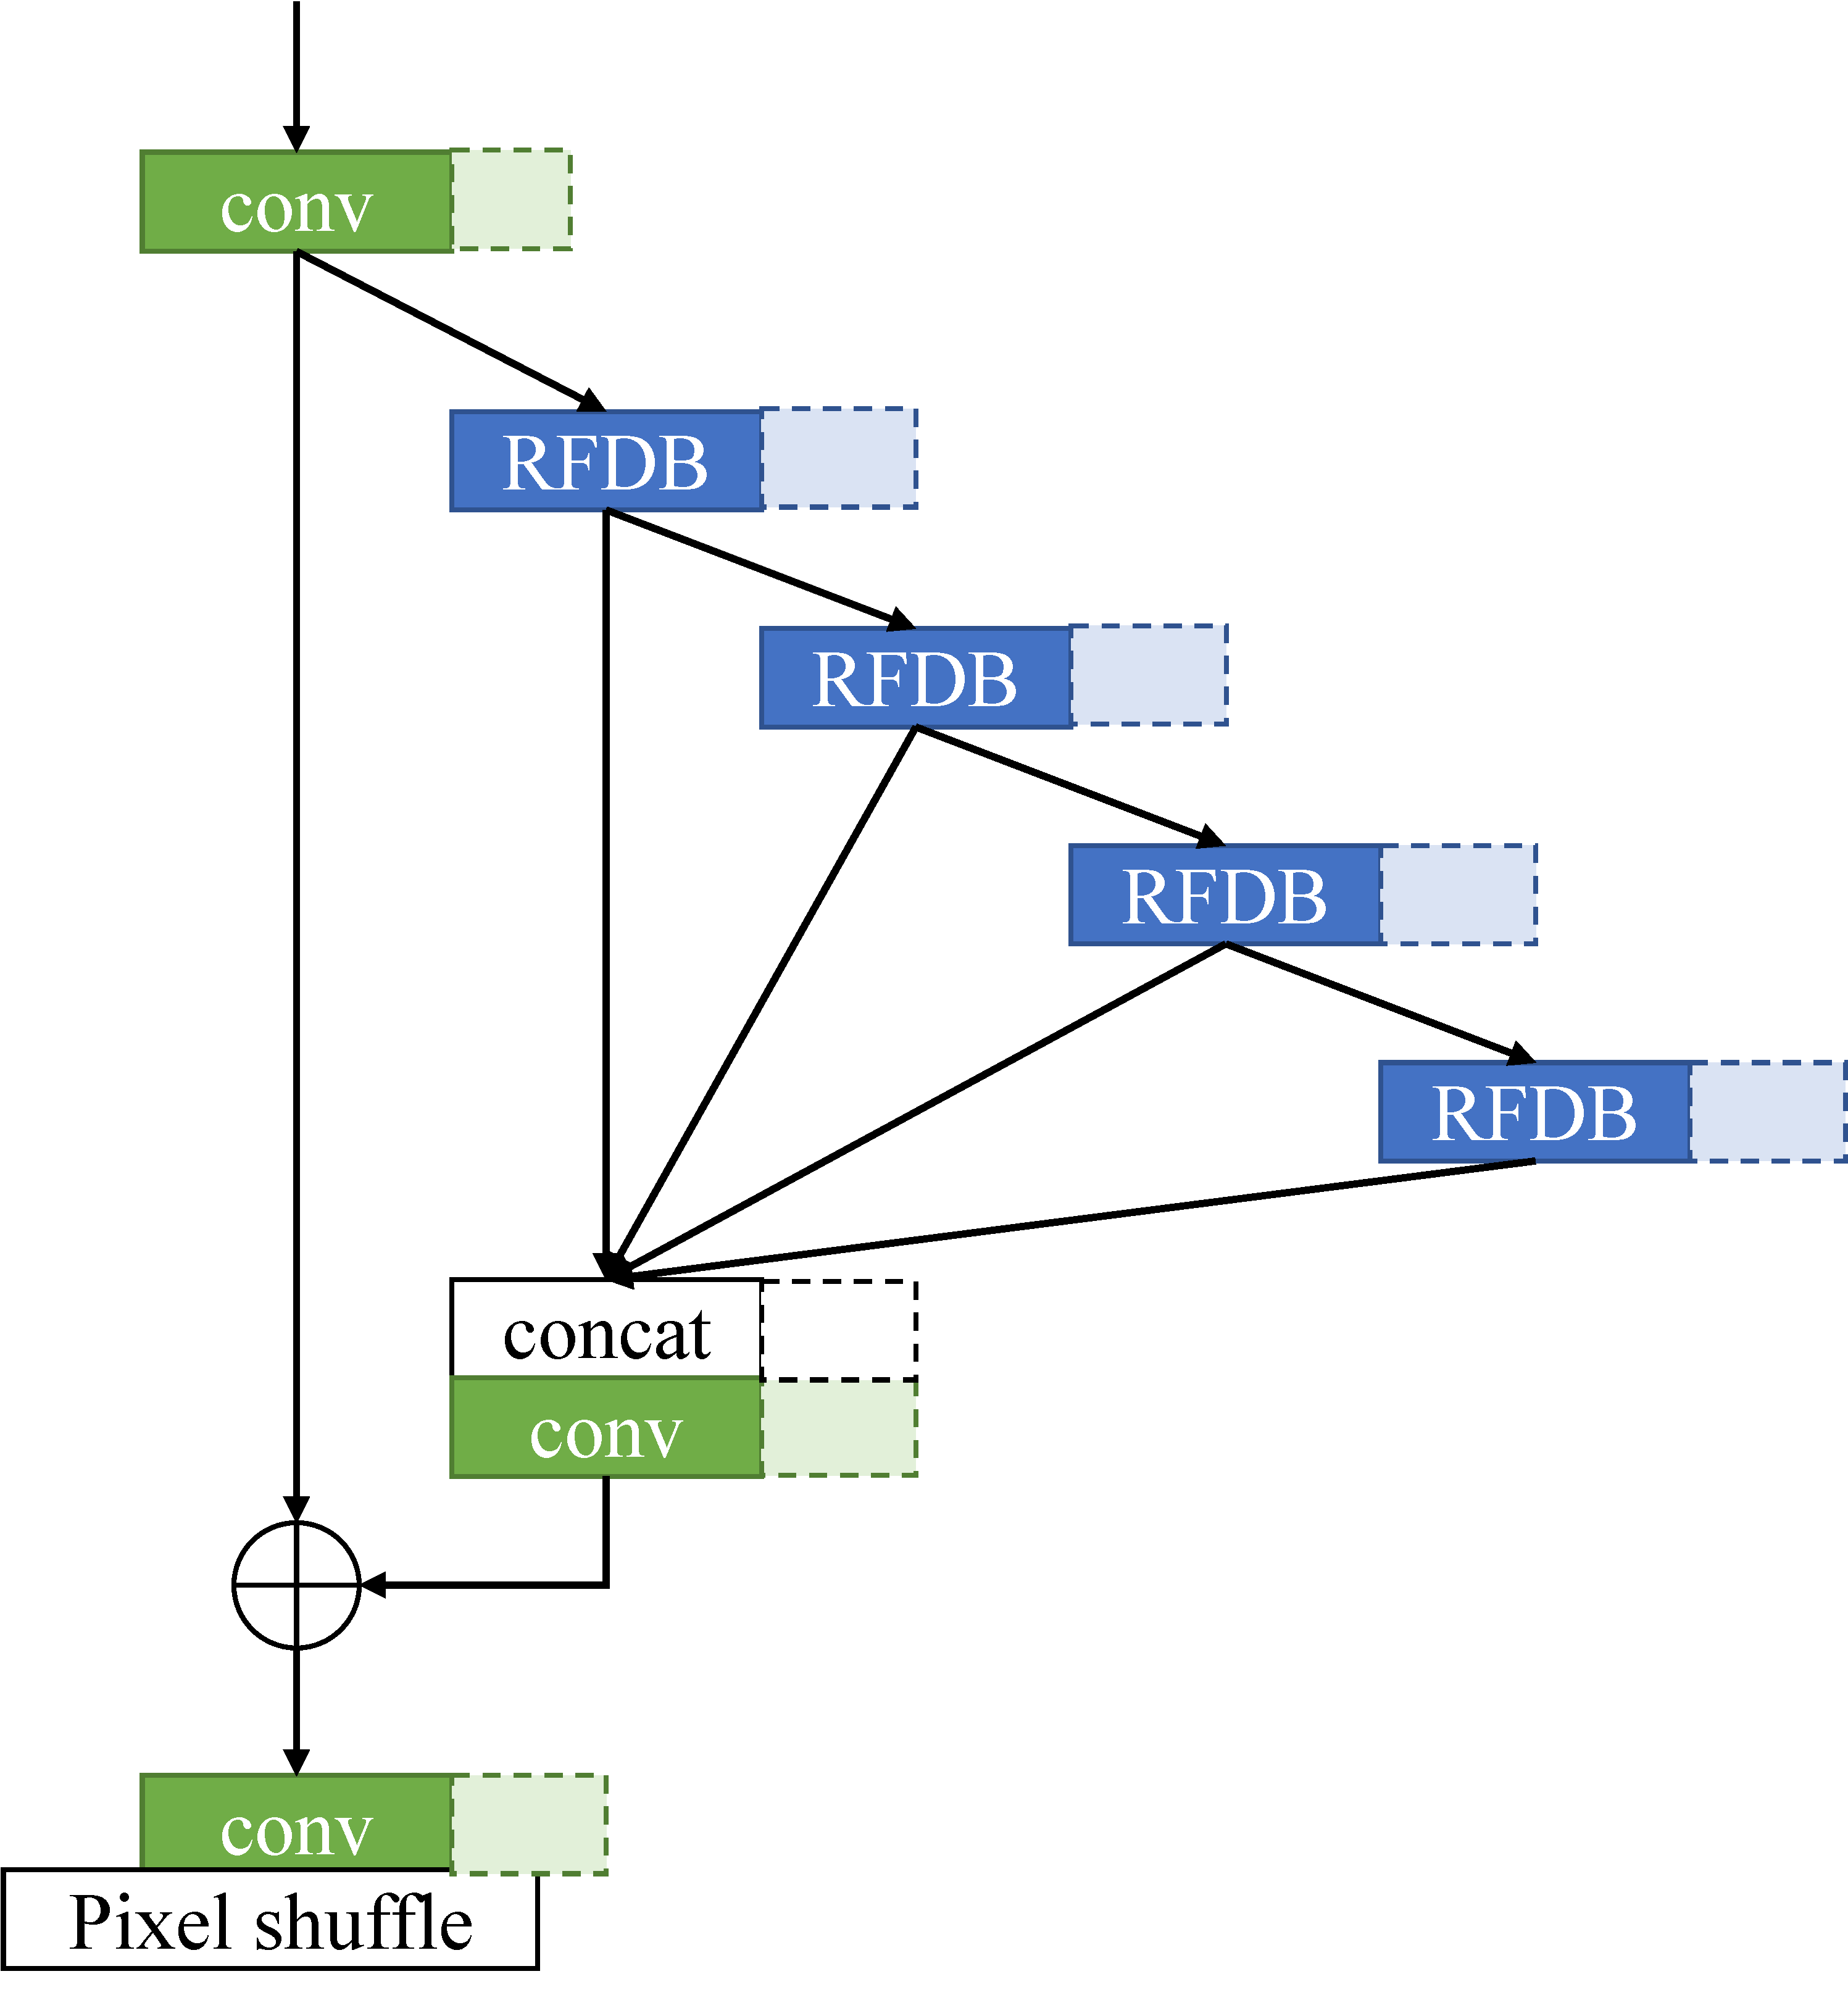
\includegraphics[width=\textwidth]{../shrink.pdf}
        \caption{Shrinking}
        \label{fig:Shrinking}
    \end{subfigure}
    \caption{Expanding and shrinking RFDN}
    \label{fig:PRFDN}
\end{figure*}

\subsection{Insights on designing efficient model.}
Lots of work focusing on designing efficient model to achieve SOTA performance on challenges year by year. A big problem under the phenomenon that collecting collect more data and create a new larger dataset for training a bigger and more powerful model is that we always need to update our model to adapt to the new dataset for learning more knowledge than before and also keep its efficiency which is always tedious.

Efficient insights are not easy to find and always ignored some important factors in the advanced computing platforms and due to good performance in theory but bad performance in reality which can happen on running MobileNet on different platforms.

We want to find a method that scaling an existing SOTA efficient model efficiently and effectively. By this way, we can just absorb achievements from efficient model design research and scale them to get a new SOTA in a new dataset.

We improve RFDN\cite{liu2020residual} model inspired on the "Train Big, Then Compress" theory proposed by \cite{li2020trainlarge} and proposed "Expand Big, Then Shrink" idea. On one hand, big model has more parameters than small model so that they can learn more knowledge from the dataset. If there is a new dataset larger than a traditional dataset which is the situation of LSDIR and DIV2K, the old SOTA model is not enough to learn new knowledge from the new large dataset, so that we need to expand it. On the other hand, a expanded model always has redundancy in computation, using compressing method to shrink it can make it efficient and without knowledge loss.

\subsection{Details}
We first expand all channels of operation in RFDN exclude pixelshuffle operation with 2x factor and then train it which is a big model training and achieved better results for its larger model capacity.
After training, a heavy compression followed.
We utilize a dynamic structure pruning method\cite{fang2023depgraph} to compress model and finetune it iteratively.

Prune and finetune description.

\subsection{Rethinking the complexity of expanding and shrinking.}

We used simple universal scaling methods to expand and shrink model structure but still achieving better accuracy-speed trade-off rather than the original model and the most of peers. On one hand, the way we used to expand model is based on width-multiplier which changed the width of all layers with a same scale. On the other hand, the way we used to shrink is a simple $\mathcal{L}1$ norm based pruner and also shrink all layers with a same scale. This result has proven the effectiveness and potency of the idea of "Expand and Shrink" scaling method.

%------------------------------------------------------------------------
\section{Experiments}
\label{sec:exp}

Experiments.

%------------------------------------------------------------------------
\section{Conclusion}
\label{sec:conclud}

Conclusion.


%%%%%%%%% REFERENCES
{\small
\bibliographystyle{ieee_fullname}
\bibliography{egbib}
}

\end{document}
